\documentclass{article}

\usepackage[preprint]{neurips_2024}

\usepackage{amsmath}  
\usepackage{amssymb}  
\usepackage{bm}     
\usepackage[utf8]{inputenc} 
\usepackage[T1]{fontenc}  
\usepackage{hyperref}     
\usepackage{url}           
\usepackage{booktabs}    
\usepackage{amsfonts}       
\usepackage{nicefrac}      
\usepackage{microtype}     
\usepackage{xcolor}     
\usepackage{float}
\usepackage{graphicx}
\graphicspath{{images/}}

\title{Tracing political discourse evolution: Topic modeling of the 1981 and 1988 French legislative elections}


\author{%
  Florian Jacquetin\thanks{ENSAE}  \\
  \texttt{florian.jacquetin@ensae.fr}
}


\begin{document}


\maketitle


\begin{abstract}
This study investigates the evolution of political discourse and communication strategies in French legislative elections between 1981 and 1988. We extract latent topics from candidates' manifestos comparing three NLP methods. The most efficient (NMF) highlights a structural transformation of the French political semantic space, moving from a relatively stable left–right opposition in 1981 to a more fragmented configuration in 1988, characterized by the emergence of a distinct extreme-right pole and increasing internal differentiation within the left.
\end{abstract}


\section{Introduction}
The analysis of political texts provides insights into party strategies and the evolution of political discourse over time. Traditional content analysis methods are often labor-intensive and limited in scope. Topic modeling, a set of unsupervised machine learning techniques, allows researchers to automatically identify the latent themes present in large corpora of text \citep{blei2003latent}. Recent advances in natural language processing (NLP), particularly transformer-based models, have enabled richer representations of text that capture contextual meaning. These methods have improved the interpretability and granularity of topics discovered in political texts \citep{grootendorst2022bertopic}.

\section{State of the art}

Early work in the field was dominated by probabilistic topic models, among which Latent Dirichlet Allocation (LDA) \citep{blei2003latent} remains the most influential. LDA models each document as a mixture of latent topics, and each topic as a distribution over words, within a fully probabilistic framework. This structure provides interpretable outputs and allows for statistical inference, which explains its widespread adoption in political science. In particular, LDA has been extensively used to analyze party manifestos, legislative debates, and political speeches, enabling systematic comparisons across parties, countries, and time periods \citep{greene2016topic}. Its probabilistic nature, compatibility with extensions such as dynamic or structural topic models, and strong integration within established research traditions have made it the dominant approach for topic extraction in political text analysis.

Alongside LDA, alternative methods such as Non-negative Matrix Factorization (NMF) \citep{lee1999nmf} have been proposed. NMF relies on a linear algebraic decomposition of the document-term matrix into non-negative factors, yielding additive representations of topics. While it does not provide a probabilistic interpretation, NMF often produces sparse and interpretable components, which can be advantageous when analyzing relatively small or noisy corpora. However, its lack of a generative framework and more limited theoretical grounding in statistical inference have contributed to its more marginal use in political science compared to LDA.

Despite their success, both LDA and NMF rely on a bag-of-words assumption, ignoring word order and contextual meaning. This limitation has motivated the development of neural approaches based on distributed representations of language. The introduction of transformer-based models such as BERT marked a major turning point, enabling the encoding of words and sentences into dense vector representations that capture semantic and contextual nuances. BERTopic \citep{grootendorst2022bertopic} represents a new generation of topic modeling techniques. It combines contextual embeddings (typically from BERT or Sentence-BERT) with dimensionality reduction (UMAP) and density-based clustering (HDBSCAN), followed by class-based TF-IDF to extract interpretable topic representations.

Empirical applications of BERTopic in political science are still emerging and remain relatively limited compared to LDA. One notable exception is the study by \citet{orellana2023nlp}, which applies BERTopic to political party manifestos in New Zealand, demonstrating its ability to extract meaningful thematic structures and complement traditional approaches. However, most existing applications of BERTopic in the political domain focus on social media data, particularly Twitter  \citep{mendonca2024twitterverse}.

\section{Pre-processing and statistics}
We chose to use the electoral manifestos (“professions de foi”) of candidates from the French legislative elections of 1981 and 1988. We restricted our analysis to first-round manifestos in order to avoid duplicate entries for candidates who advanced to subsequent rounds, and to construct a dataset that is as representative as possible of the full range of political parties active during that period. In a second step, we lemmatized the textual data and associated each manifesto with the political party supporting the candidate. We standardized party names—addressing inconsistencies such as capitalization and alternative spellings or acronyms—in order to retain the ten main political parties in 1981: the French Communist Party, the Socialist Party, Lutte Ouvrière, the Unified Socialist Party, the Rally for the Republic, the Union for French Democracy, the Radical Party of the Left, the National Front, the Revolutionary Communist League, and the Party of New Forces. In cases of coalitions, we assigned the manifesto to the first party listed, which typically corresponds to the leading party within the alliance. All other, less represented parties were grouped into a residual “Others” category. Eventually, we then used SpaCy to lemmatize the text and removed non-French content, in particular German-language manifestos found in regions such as Alsace-Lorraine.

\begin{table}[H]
\centering
\begin{tabular}{lccc}
\hline
\textbf{Step} & \textbf{1981} & \textbf{1988} & \textbf{Total} \\
\hline
Documents initially loaded & 3182 & 3628 & 6810 \\
First-round manifestos retained & -- & -- & 5102 \\
Documents containing German text removed & -- & -- & 102 \\
Final number of manifestos & -- & -- & 4982 \\
\hline
\end{tabular}
\caption{Summary of data processing steps}
\end{table}

\begin{figure}[htbp]
    \centering
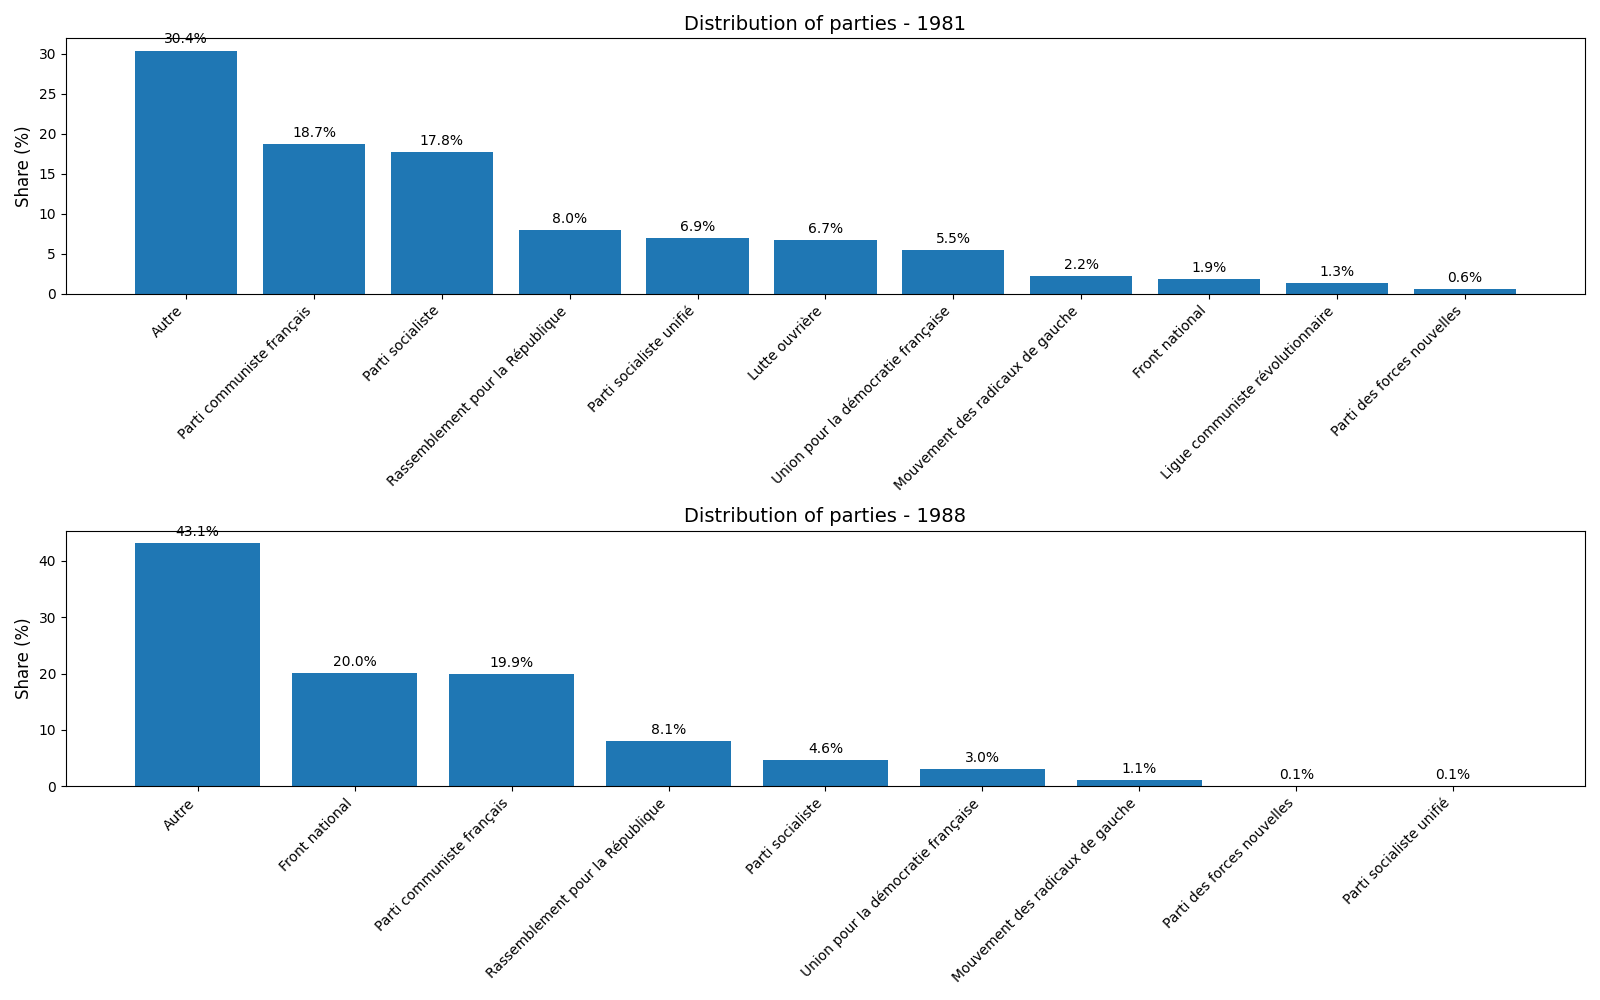
\includegraphics[scale=0.38]{parti.png}
    \caption{Parties' distribution}
    \label{fig:parti}
\end{figure}


\section{Metrics}

Following \citet{grootendorst2022bertopic}, we use \textbf{topic coherence} and \textbf{topic diversity} to jointly assess interpretability and redundancy.

\paragraph{Topic coherence.}
Let a topic $k$ be defined by its top-$M$ words $W_k = \{w_1, \dots, w_M\}$. Using Normalized Pointwise Mutual Information (NPMI):
\begin{equation}
\text{NPMI}(w_i, w_j) = \frac{\log \frac{P(w_i, w_j)}{P(w_i)P(w_j)}}{-\log P(w_i, w_j)},
\end{equation}
the coherence of topic $k$ is: $C(k) = \frac{2}{M(M-1)} \sum_{i<j} \text{NPMI}(w_i, w_j)$
and overall coherence is: $C = \frac{1}{K} \sum_{k=1}^K C(k)$


\paragraph{Topic diversity.}
Let $W = \bigcup_{k=1}^K W_k$. Diversity is: $D = \frac{|W|}{KM}$.

We define a final score as the product $C \times D \in [0,1]$, combining semantic quality (coherence) and non-redundancy (diversity).

\section{Models, grid search and hyperparameters}

\subsection{BERTopic}
Following the approach of \citet{orellana2023nlp} and \citet{mendonca2024twitterverse}, we apply NLP techniques to identify the topics discussed by political parties. We implement the method proposed by \citet{grootendorst2022bertopic}, which combines sentence transformers with a variant of TF-IDF called class-based TF-IDF (c-TF-IDF) to generate clusters of interpretable topics. Documents with similar topics are first projected into a lower-dimensional space using UMAP (Uniform Manifold Approximation and Projection), which facilitates clustering. After this dimensionality reduction, the documents are grouped using HDBSCAN (Hierarchical Density-Based Spatial Clustering of Applications with Noise). Finally, we employ the BERTopic model from the Python package by Grootendorst, which leverages embeddings derived from Sentence-BERT.

UMAP requires three hyperparameters: the number of neighbors, the number of principal components and the minimum distance (we use a \textit{cosine} metric. HDBSCAN needs a cluster size minimum.

These four hyperparameters —are optimized via a grid search based on topic coherence and topic diversity. The grid search explores the following ranges: number of components from 2 to 4, number of topics from 10 to 20, and number of neighbors from 10 to 20. Following \citet{orellana2023nlp}, our default settings use the top 10 words per topic and a minimum topic size of 10. A one-dimensional n-gram representation is sufficient, as BERTopic captures multi-word expressions effectively through sentence embeddings. Coherence is maximized for the following hyperparameter combination: 4 components, 19 neighbours, a minimum distance of 0.3 and minimum cluster size of 19  (see Table \ref{app:grid_bert}).

\subsection{NMF}

We also implement Non-Negative Matrix Factorization (NMF) as an alternative topic modeling approach. NMF decomposes the document-term matrix obtained via TF-IDF into two non-negative matrices: one representing document-topic associations and the other topic-term associations. Each topic is represented by a weighted combination of terms, which allows for semantic interpretation. Unlike probabilistic models, NMF does not assume an underlying generative process, but it has been shown to produce coherent and interpretable topics, particularly when using TF-IDF weighting. We construct the document-term matrix using a TF-IDF vectorizer with a minimum document frequency of 0.5\% and a maximum of 70\%, and consider n-grams of size 1 or 2. The number of topics is treated as a hyperparameter, tuned to maximize the score defined as topic coherence $\times$ topic diversity. Grid search over the number of topics (ranging from 8 to 20) and n-gram ranges ((1,1) and (1,2)) identifies the optimal configuration (see Table \ref{app:grid_nmf}. Topics are visualized both as lists of top words and as heatmaps representing the average topic distribution per political party. We eventually select $n_{topic} = 14$ to avoid some redundant topics.

\subsection{LDA}

Finally, we apply Latent Dirichlet Allocation (LDA) \citep{blei2003latent} to model the political discourse. LDA is a generative probabilistic model that assumes each document is a mixture of latent topics, and each topic is a distribution over words. Unlike NMF, LDA explicitly models uncertainty and provides document-level topic probabilities, making it suitable for analyzing overlapping topics and subtle variations in discourse. We fit LDA on a matrix of word counts. The key hyperparameters—the number of topics and the Dirichlet priors on document-topic and topic-word distributions—are optimized using the score  (see Table \ref{app:lda_grid}).

\section{Results}

\subsection{BERTopic}
We restrict the analysis to six topics, as a larger number tends to generate redundant and less interpretable themes. Since BERTopic assigns a single dominant topic to each document, the majority of texts are classified under the topic related to positioning toward the socialist presidential majority.

\begin{table}[htbp]
\centering
\small
\begin{tabular}{@{} l p{10cm} @{}}
\toprule
\textbf{Topics} & \textbf{Top words} \\
\midrule
Majorité présidentielle & majorit, communiste, falloir, homme, prsident, rpublique, changement, monsieur, donner, 14 \\
Critique financière & accepter, triage, illusion, sortir, financier, production, dtruire, technologie, temps, celer \\
Opposition de droite & conviction, suppression, liste, redressement, fiscalist, lepen, payent, 4400000, antisocialiste, absent \\
Economie et travail & engager, degr, pourcent, chmeur, doubler, comptitivit, production, aller, million, 1992 \\
Revendications sociales & lcr, travailleur, unit, revendication, patron, falloir, giscard, communiste, prendre, ministre \\
Fiscalité & conviction, liste, suppression, penscience, fiscalist, 4400000, gard, octroi, hgmonie, maternel \\
\bottomrule
\end{tabular}
\caption{Topics (BERTopic) identified and their top words.}
\label{tab:topics_summary}
\end{table}

\begin{figure}[htbp]
    \centering
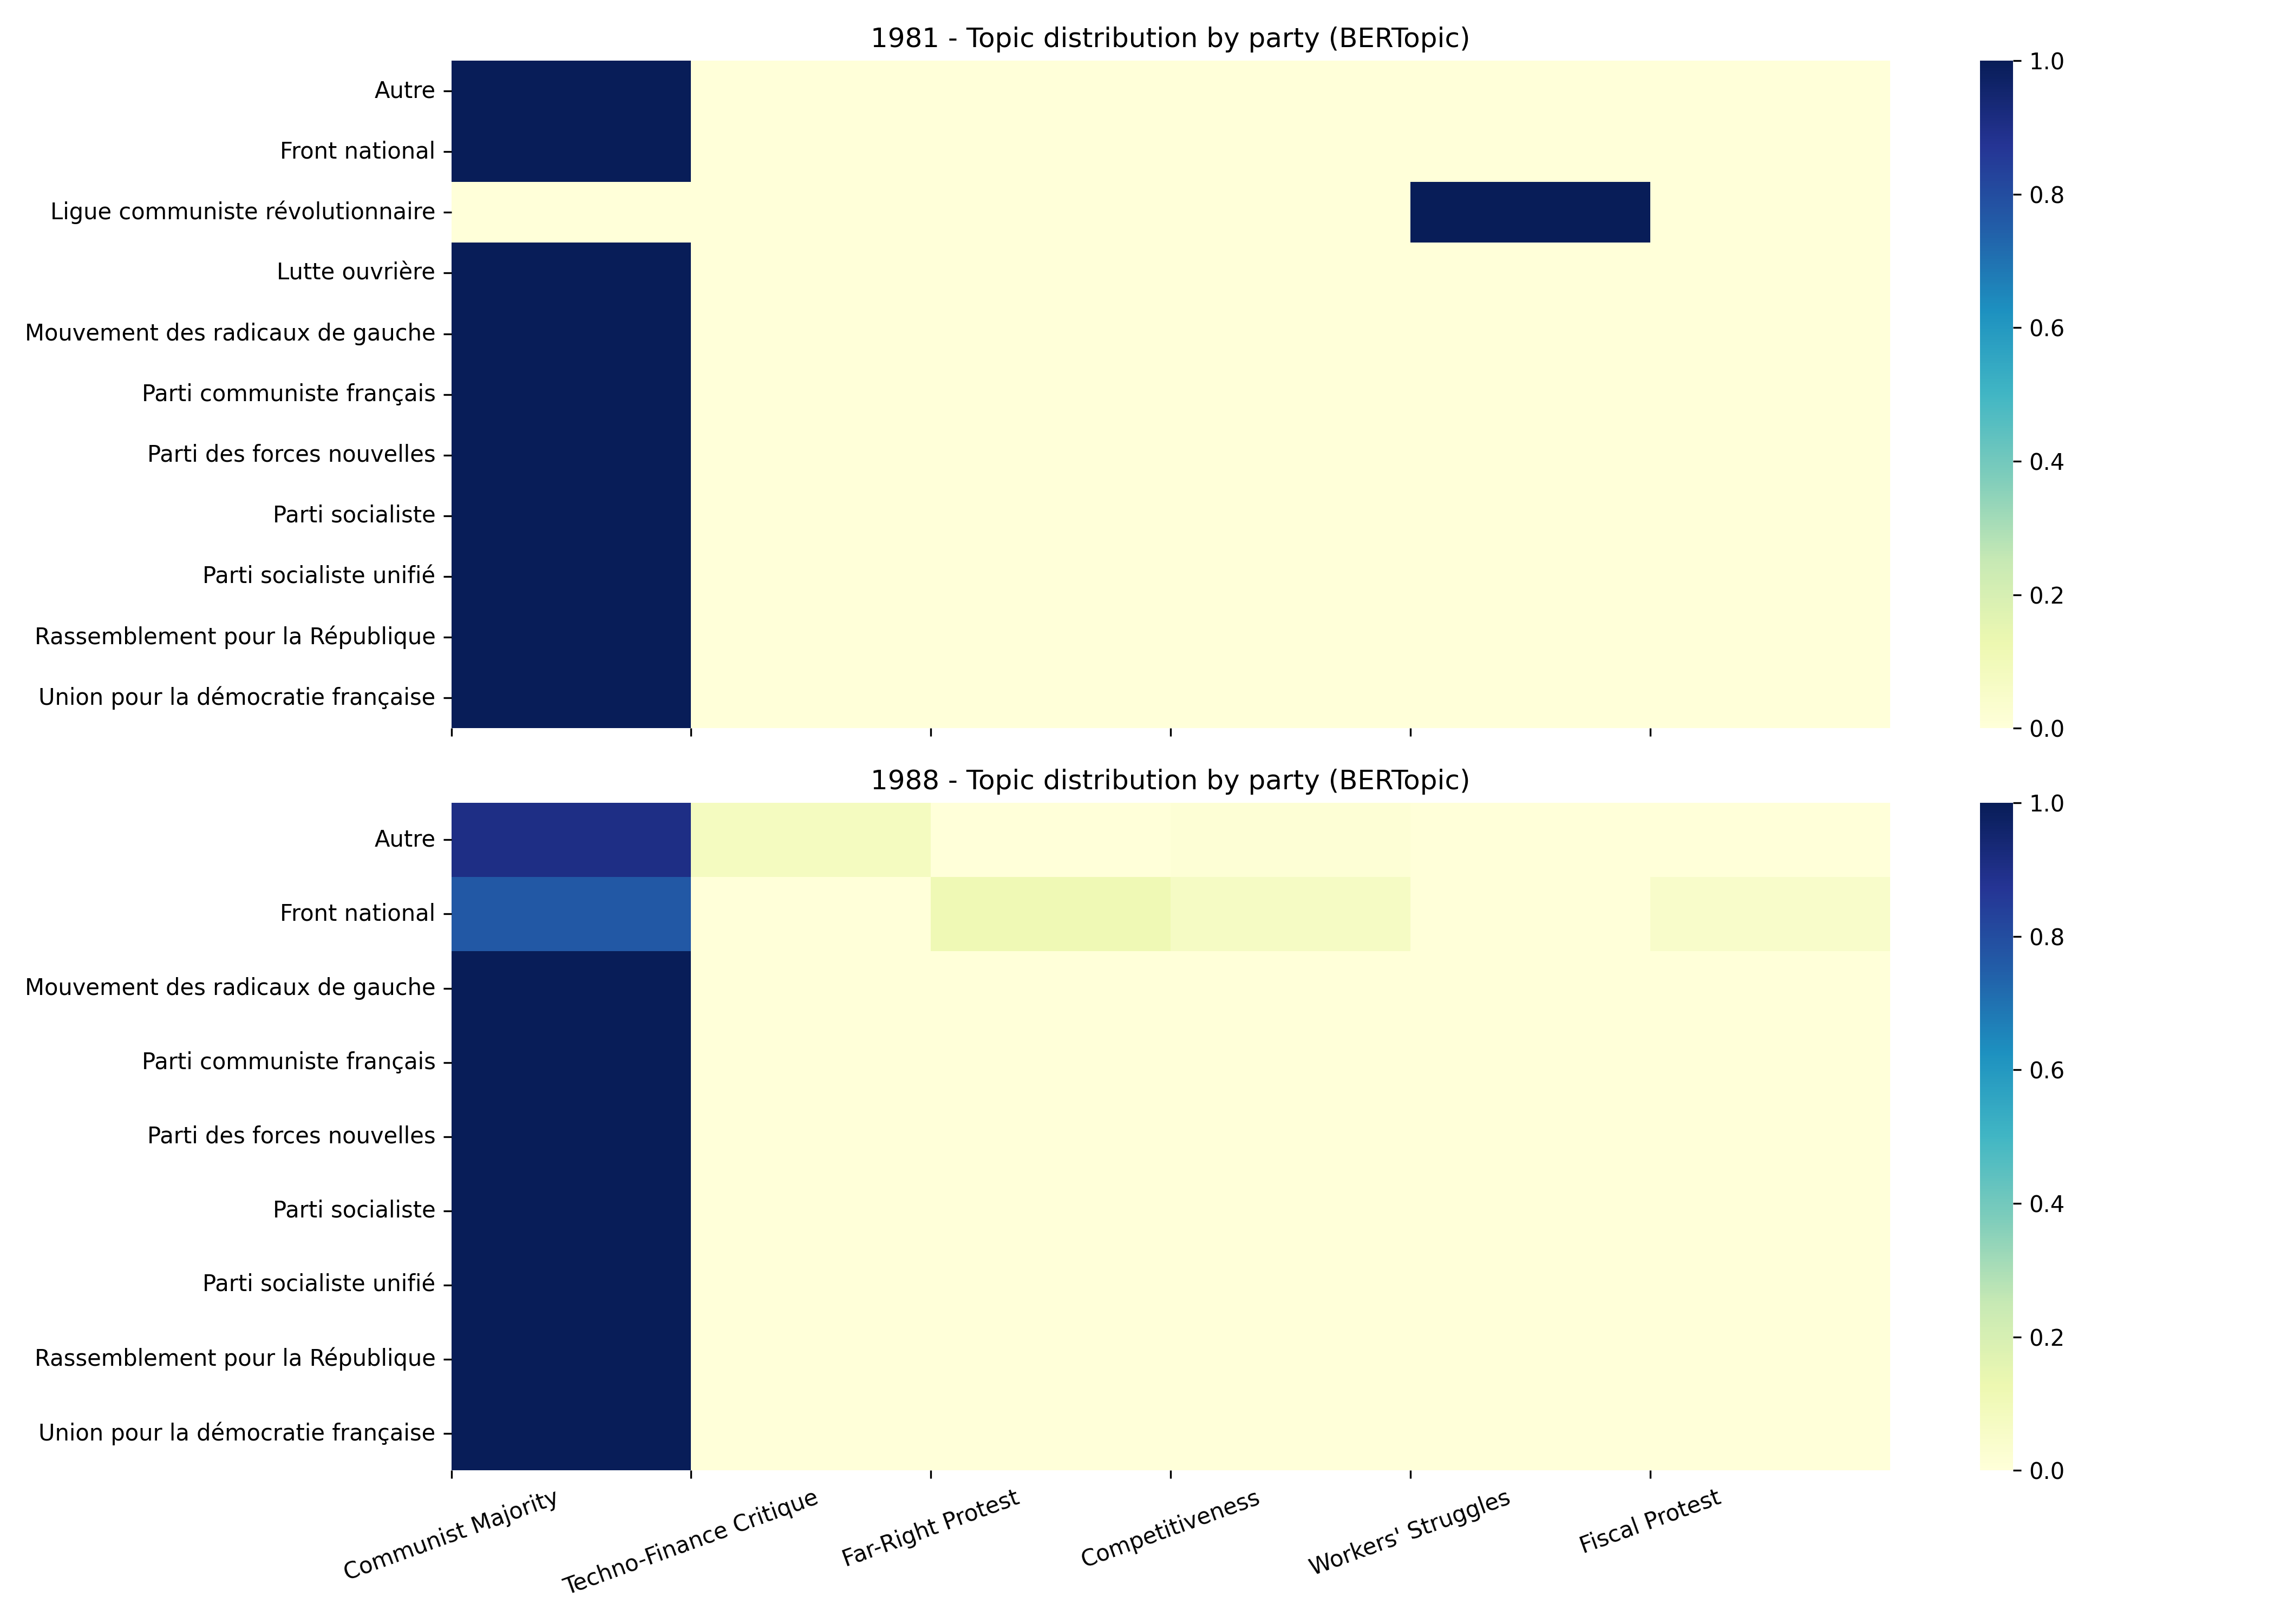
\includegraphics[scale=0.5]{bert_results.png}
    \caption{BERTopic results}
    \label{fig:bert_results}
\end{figure}


\subsection{NMF}
Among the 14 topics, several interesting evolutions can be observed between 1981 and 1988. In 1981, the Socialist Party leveraged the momentum from Mitterrand's election to consolidate a parliamentary majority. By 1988, this topic had largely disappeared, as the party shifted its focus toward defending French union and solidarity, drawing on lessons from its first term in office. The Communist Party, which acted as a left-wing ally in 1981, initially focused on broader leftist mobilization. Following a period of misalignment with its allies, by 1988 it prioritized defending social gains and mobilizing its own base. The RPR and UDI exhibit similar profiles in both 1981 and 1988. In 1981, their discourse was balanced and centered on economics and labor issues. By 1988, they increasingly emphasized local governance experience and practical achievements. Eventually, the Front National emerged more prominently in 1988, articulating a distinctive discourse and expanding its number of candidates.  


\begin{table}[htbp]
\centering
\fontsize{8.5}{10}\selectfont
\begin{tabular}{@{} l p{10cm} @{}}
\toprule
\textbf{Topics} & \textbf{Top words} \\
\midrule
Extrême droite & front | front national | rpr udf | vote | rpr | udf | électeur | liste | conviction \\
Économie \& travail & devoir | travail | droit | entreprise | développement | vie | pourcent | économique | falloir | aide \\
Gauche ouvrière & travailleur | gauche | lutte ouvrière | lutte | ouvrière | laguiller | mitterrand | arlette | arlette laguiller | falloir voter \\
Pouvoir \& finance & accepter | pouvoir accepter | triage | illusion | sortir | europe | détruire | technologie | financier | production \\
Mobilisation gauche & aller | monsieur | dimanche juin | gauche politique | gauche | extrême | dimanche | besoin être | besoin | rassemblement gauche \\
Liberté \& socialisme & liberté | socialiste | 14 | majorité | 14 juin | société | union majorité | oui | président | changement \\
Écologie \& énergie & écologiste | écologie | nucléaire | écologiste battre | classe politique | énergie | démocratie | ecologie | proportionnel | économie \\
France Unie \& solidarité & france unie | unie | michel rocard | solidarité | michel | exclusion | rocard | majorité | françois | france uni \\
Patriotisme & patrie | liberté patrie | front populaire | front | public | liberté | enseignement | rassemblement liberté | rigoureux | catastrophique \\
PSU \& autogestion & psu | autogestion | nucléaire | gauche | femme | populaire | entrer homme | énergie | hiérarchie | huguette \\
Majorité présidentielle & socialiste | majorité france | parti socialiste | ensemble | donnon | 10 mai | président | majorité | 10 | françois mitterrand \\
LCR \& revendications & lcr | travailleur | candidat lcr | unité | patron | lcr être | satisfaire revendication | revendication | pc | ps pc \\
Parti communiste & communiste | gauche | rassemblement gauche | parti communiste | parti | milliard | politique gauche | candidat rassemblement | communiste français | rassemblement \\
Administration locale & maire | conseiller | général | conseiller général | centre | union rassemblement | rassemblement centre | union | président | conseil \\
Communistes \& changement & communiste | changement | gauche | réussir | majorité | victoire | réussir changement | parti communiste | union gauche | 10 mai \\
Gouvernement \& majorité & majorité | gouvernement | risque voir | gouvernement majorité | mai donner | candidat majorité | prendre risque | majorité présidentiel | pouvoir prendre | ouverture \\
\bottomrule
\end{tabular}
\caption{Topics and top words (NMF)}
\label{tab:nmf_topics}
\end{table}

\begin{table}[htbp]
\centering
\fontsize{8.5}{10}\selectfont
\begin{tabular}{@{} l p{10cm} @{}}
\toprule
Topics & Top words \\
\midrule
Majorité présidentielle & majorité | mitterrand | françois | françois mitterrand | socialiste | président | mai | république | unie | donner \\
Lutte de gauche & gauche | mitterrand | lutte | falloir | travailleur | député | majorité | gouvernement | homme | même \\
Patriotisme & liberté | national | public | front | enseignement | majorité | patrie | devoir | populaire | battre \\
Ecologie & nucléaire | écologiste | gauche | devoir | énergie | falloir | femme | travail | vie | populaire \\
Union de la gauche & communiste | gauche | parti | parti communiste | changement | majorité | union | monsieur | voix | gouvernement \\
Extrême droite & national | vote | front national | député | avenir | électeur | front | conviction | liste | confiance \\
Action parlementaire & falloir | réussir | blée | assem | assem blée | majorité | blée national | victoire | place | communiste \\
Progressisme & liberté | socialiste | majorité | union | 14 | 1981 | société | vouloir | national | 14 juin \\
Finance & accepter | europe | grand | pouvoir accepter | celer | financier | temps | illusion | production | triage \\
Economie & droit | 000 | pourcent | salaire | entreprise | travail | chômage | grand | retraite | milliard \\
Revendications sociales & travailleur | falloir | communiste | lcr | parti | ps | unité | revendication | pc | giscard \\
Droite & rpr | udf | rpr udf | front | front national | national | marie | jean marie | drogue | être front \\
Administration locale & devoir | conseiller | maire | homme | député | général | président | national | falloir | grand \\
\bottomrule
\end{tabular}
\caption{Topics and top words (LDA)}
\label{tab:lda_topics}
\end{table}

\begin{figure}[htbp]
    \centering
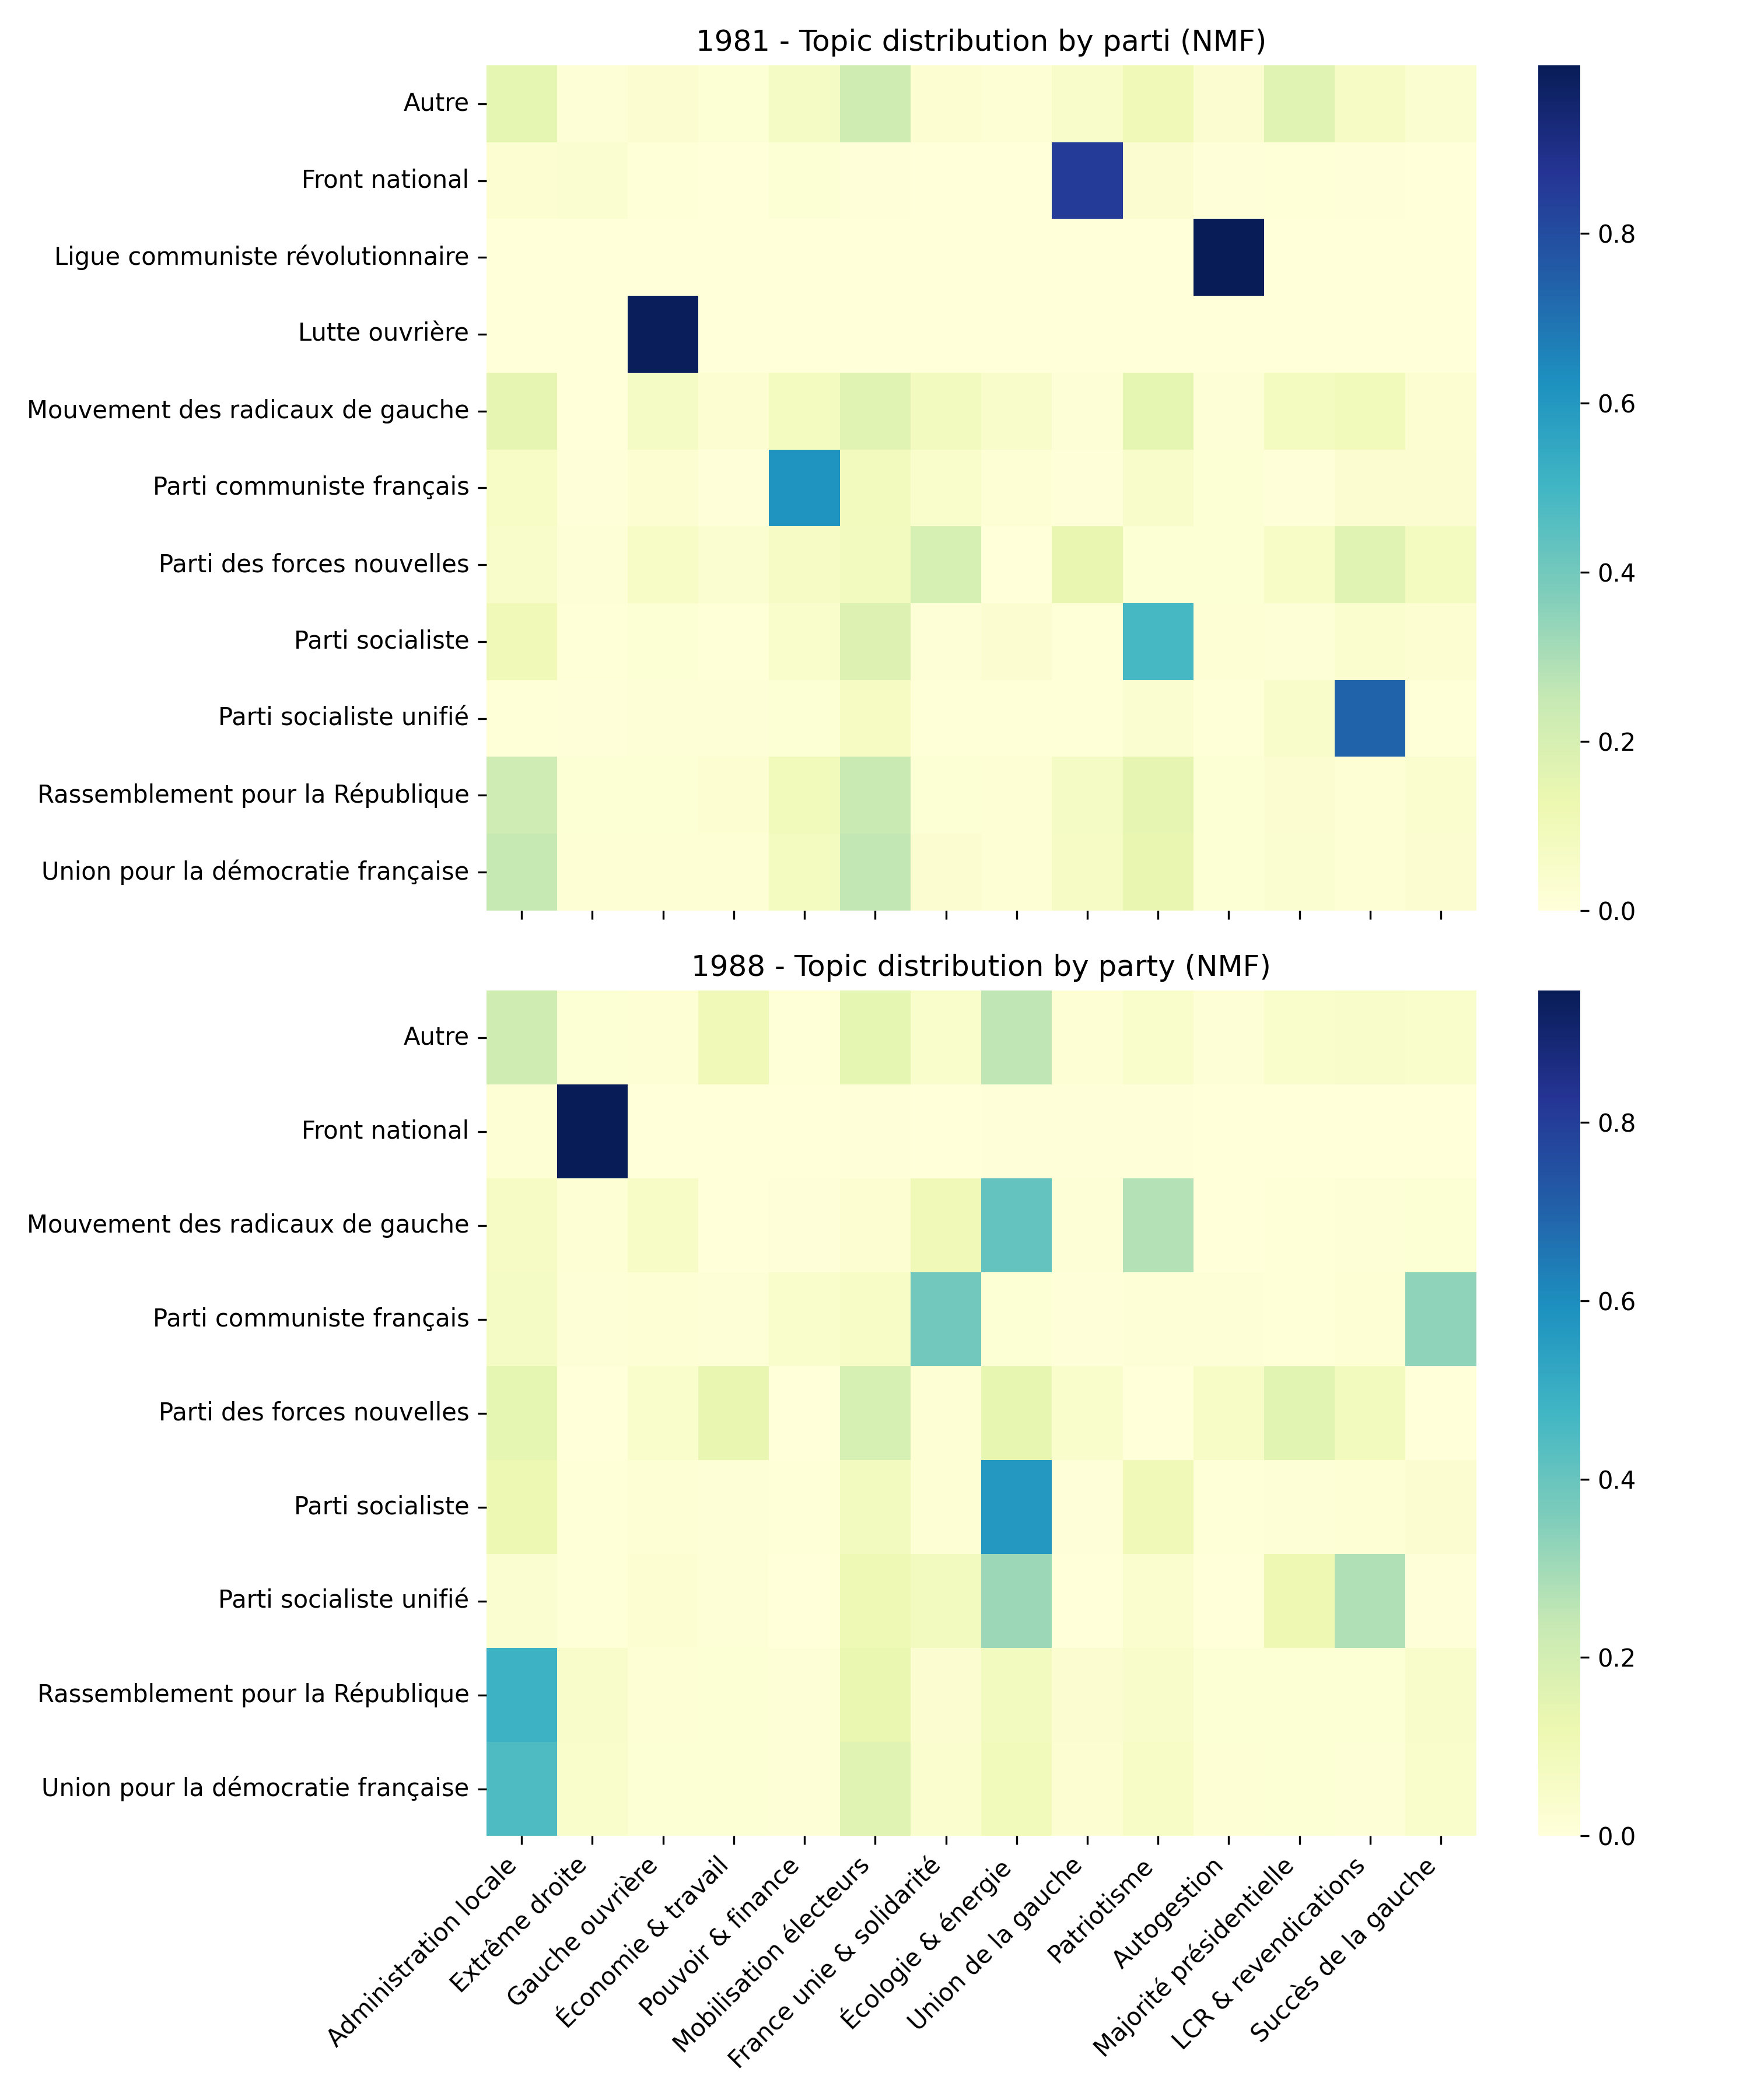
\includegraphics[scale=0.59]{nmf_results.png}
    \caption{NMF results}
    \label{fig:nmf_results}
\end{figure}

\subsection{LDA}
Among the 13 topics identified by the LDA model, we observe patterns broadly similar to those obtained with NMF. In particular, there is a noticeable shift among traditional right-wing parties from a discourse focused on mobilizing their electoral base in 1981 toward a greater emphasis on local administrative experience in 1988. More generally, most parties appear to adopt a more locally oriented discourse in 1988.

The Front National stands out as an exception. While its discourse in 1981 was more broadly patriotic, by 1988 it becomes more clearly aligned with a far-right ideological positioning, with themes that are more specific to its political identity.

However, LDA does not capture as clearly the transformations observed on the left. In contrast to the NMF results, it fails to fully identify the shift from a discourse centered on left-wing unity toward a broader narrative of national cohesion for the Socialist Party, as well as the reorientation of the Communist Party toward defending social achievements and mobilizing its own electorate.

\begin{figure}[htbp]
    \centering
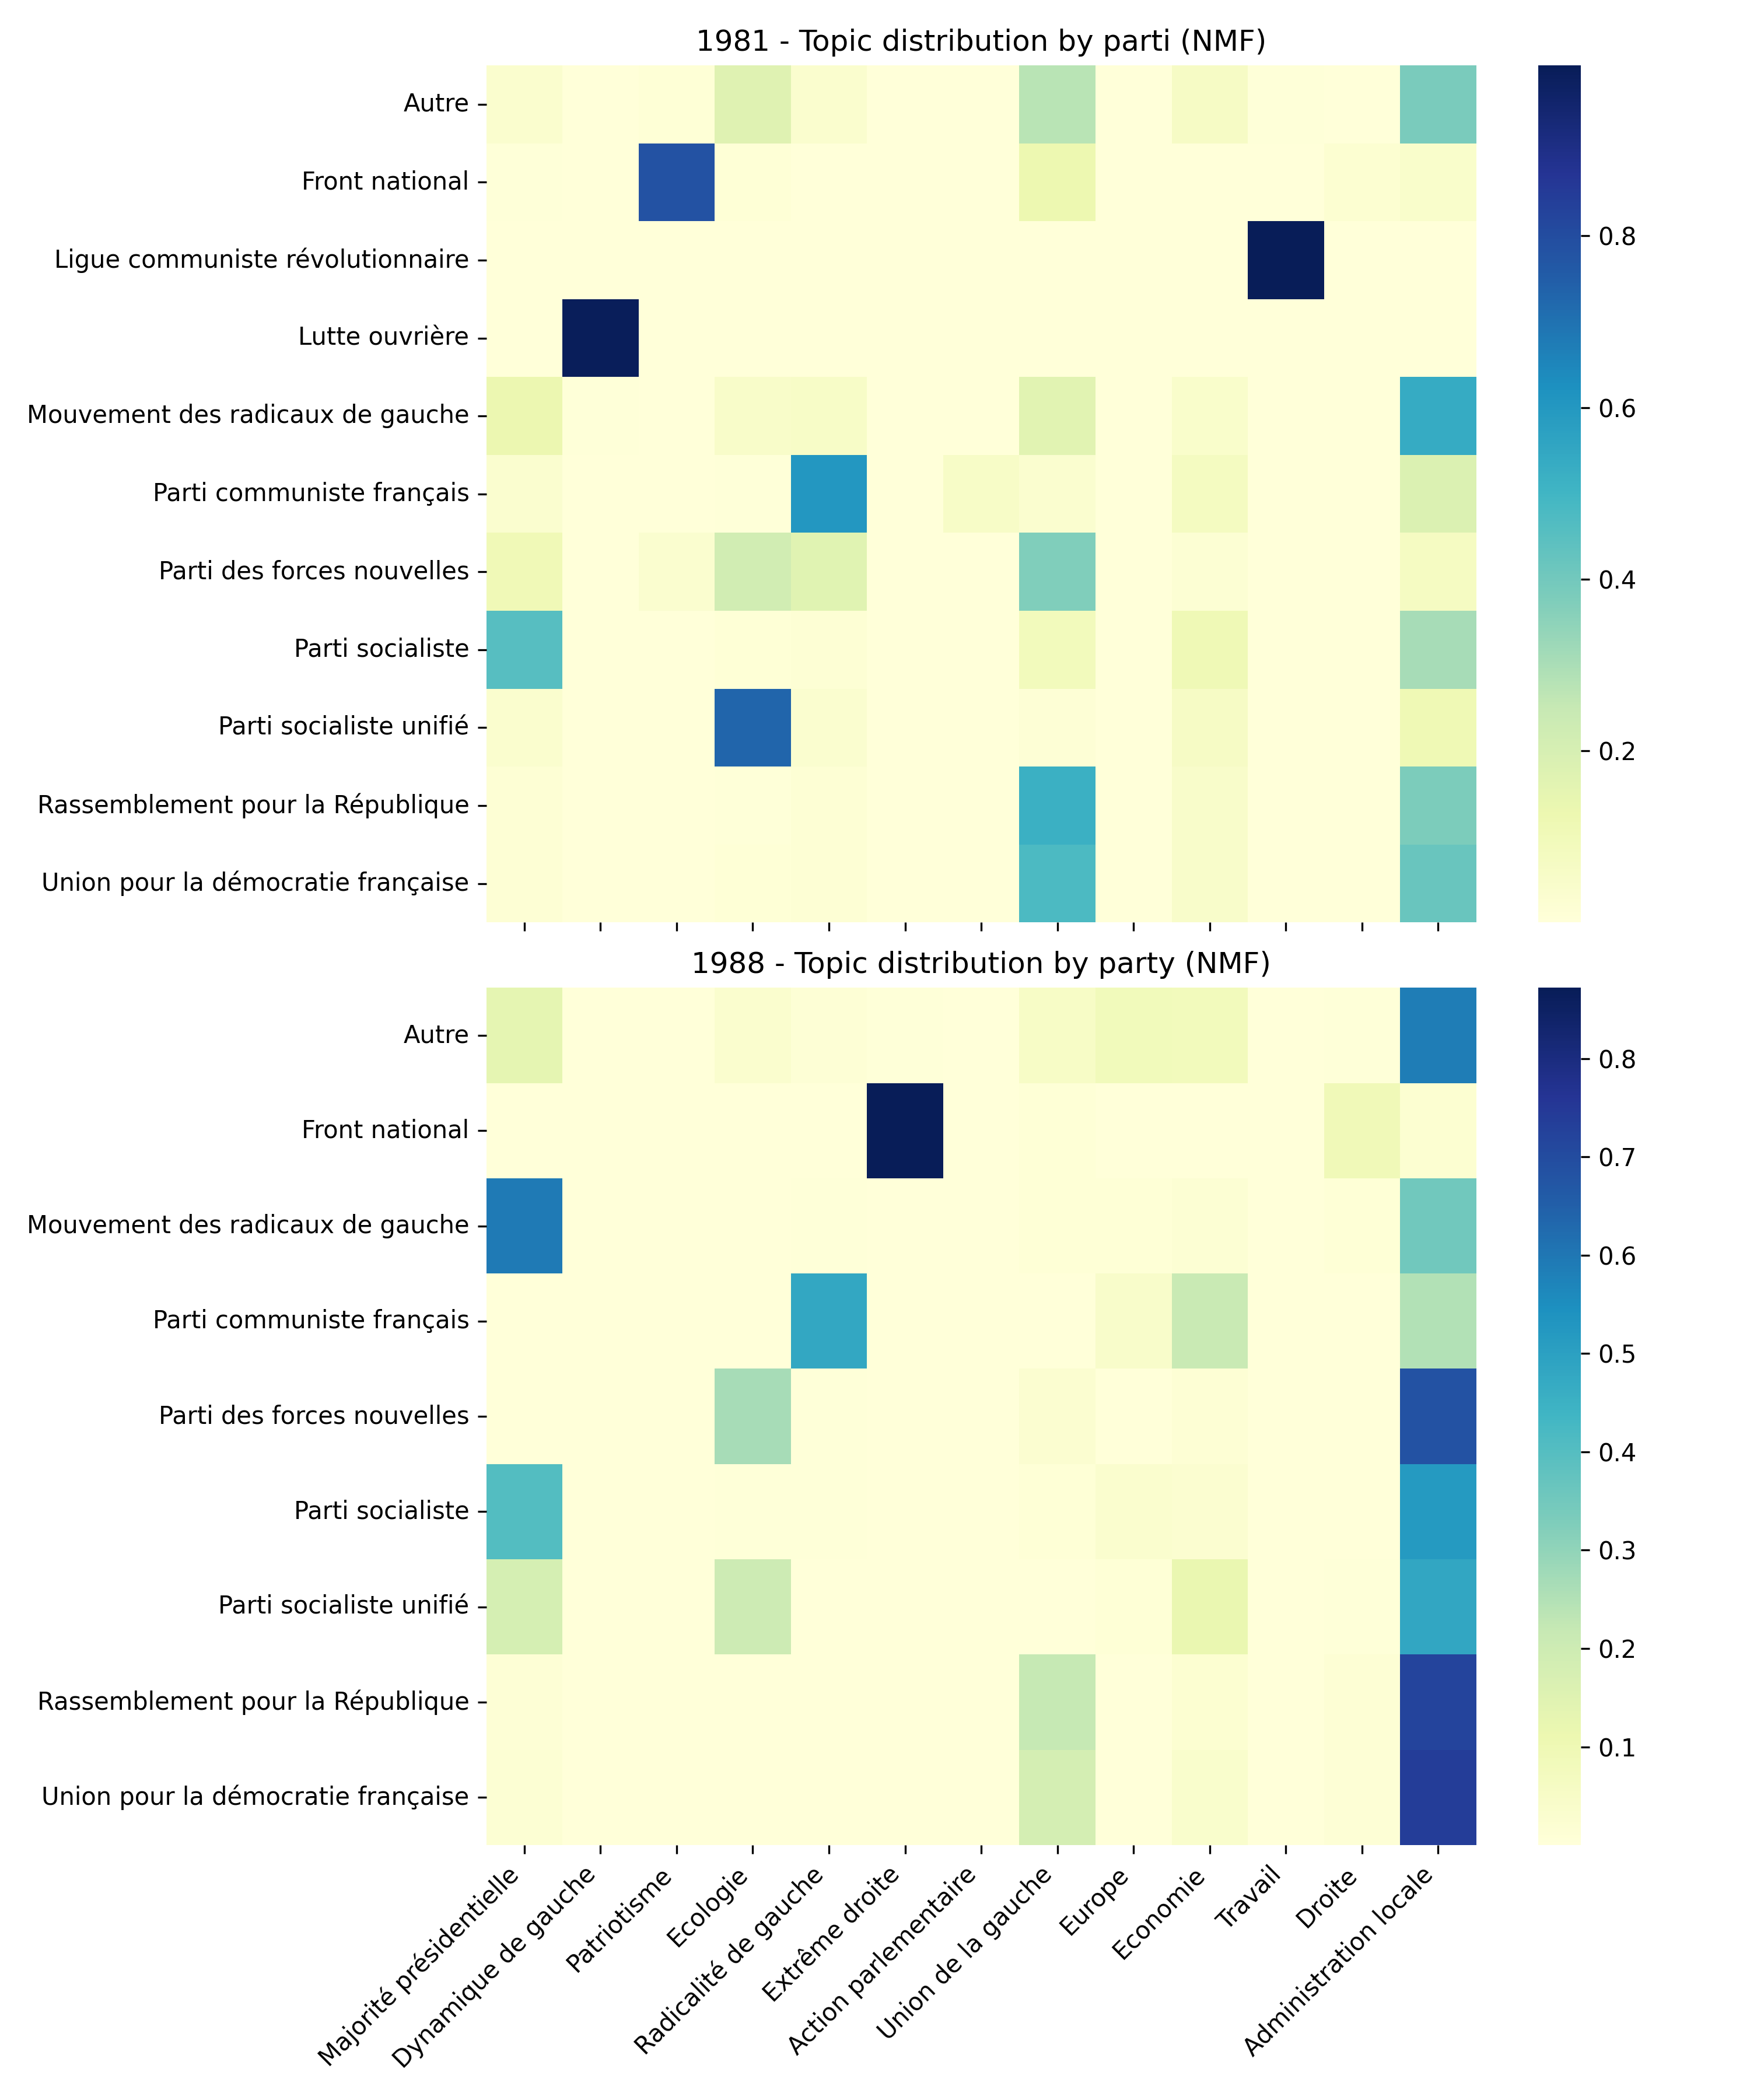
\includegraphics[scale=0.59]{lda_results.png}
    \caption{LDA results}
    \label{fig:lda_results}
\end{figure}

\section{Evolution of the semantic mapping (1981--1988)}

We study the evolution of political discourse (1981--1988) using a two-step approach. First, a NMF model on party manifestos extracts $K=14$ latent topics, interpreted as thematic dimensions. Second, a PCA is applied to party-level average topic distributions. Topic projections are shown in Figure~\ref{fig:topics}.

\begin{figure}[htbp]
    \centering
    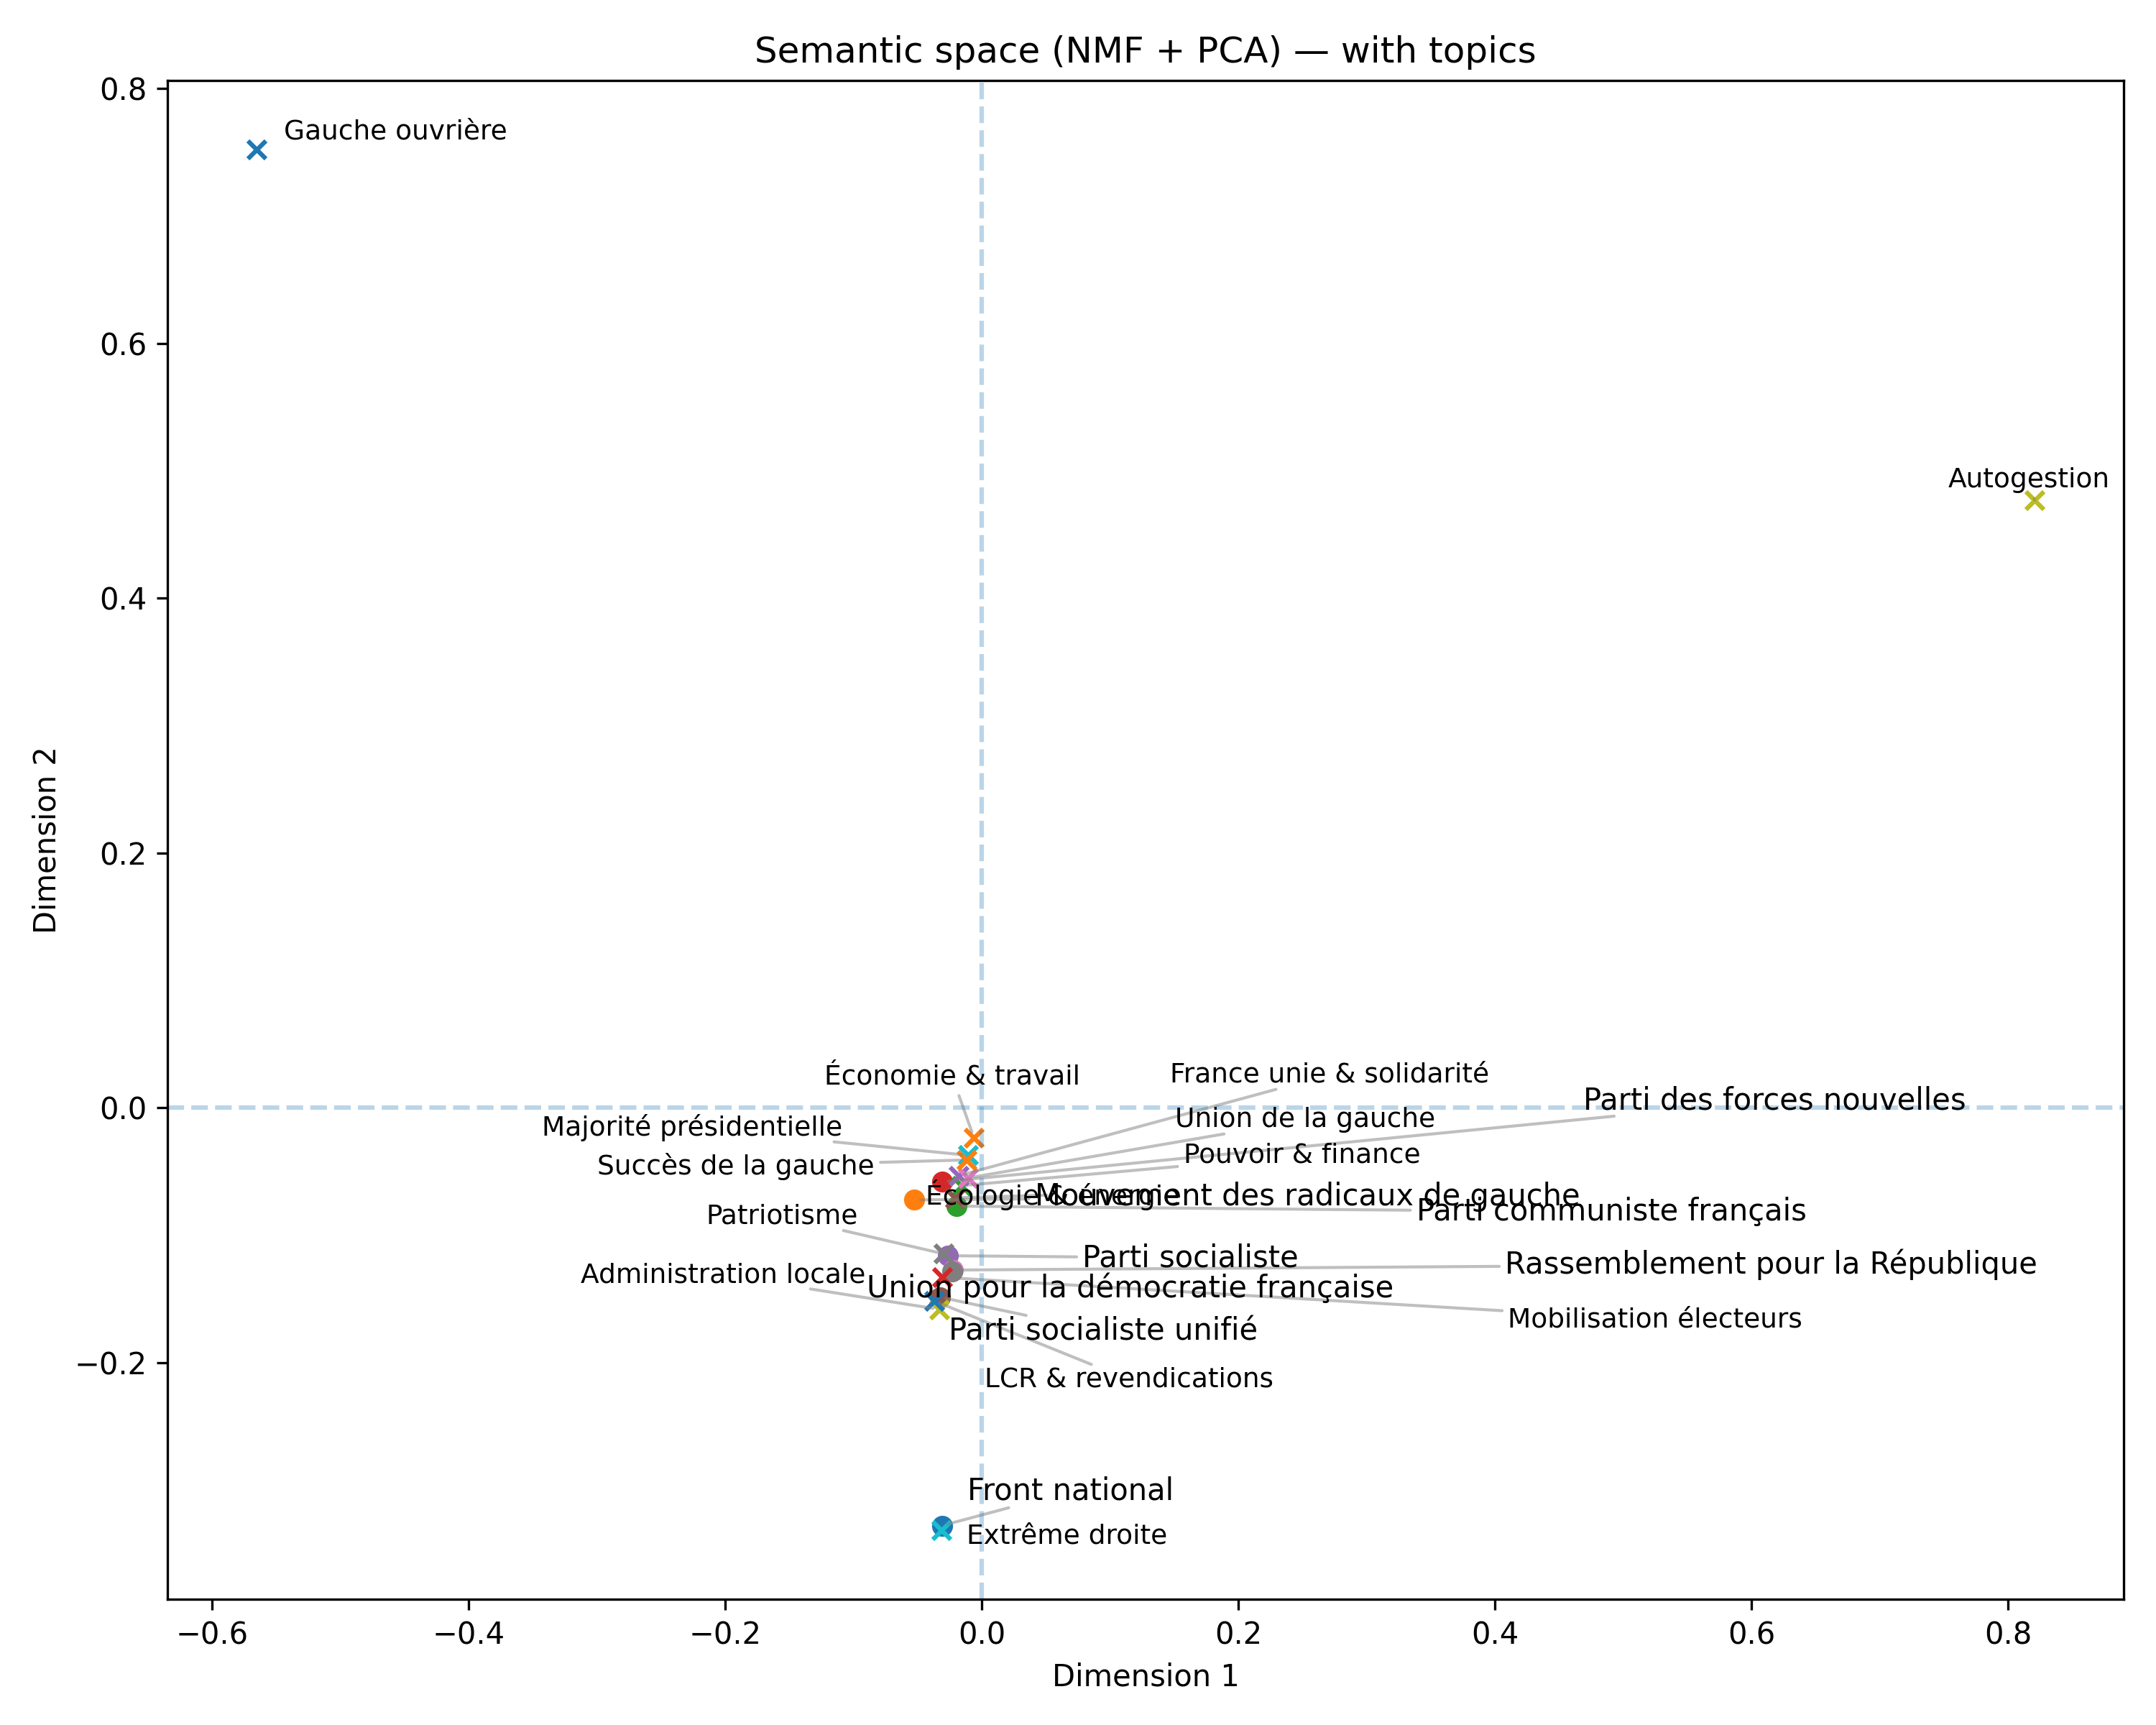
\includegraphics[width=0.8\linewidth]{nmf_pca_topic.png}
    \caption{Projection of topics in the PCA space}
    \label{fig:topics}
\end{figure}

\begin{figure}[htbp]
    \centering
    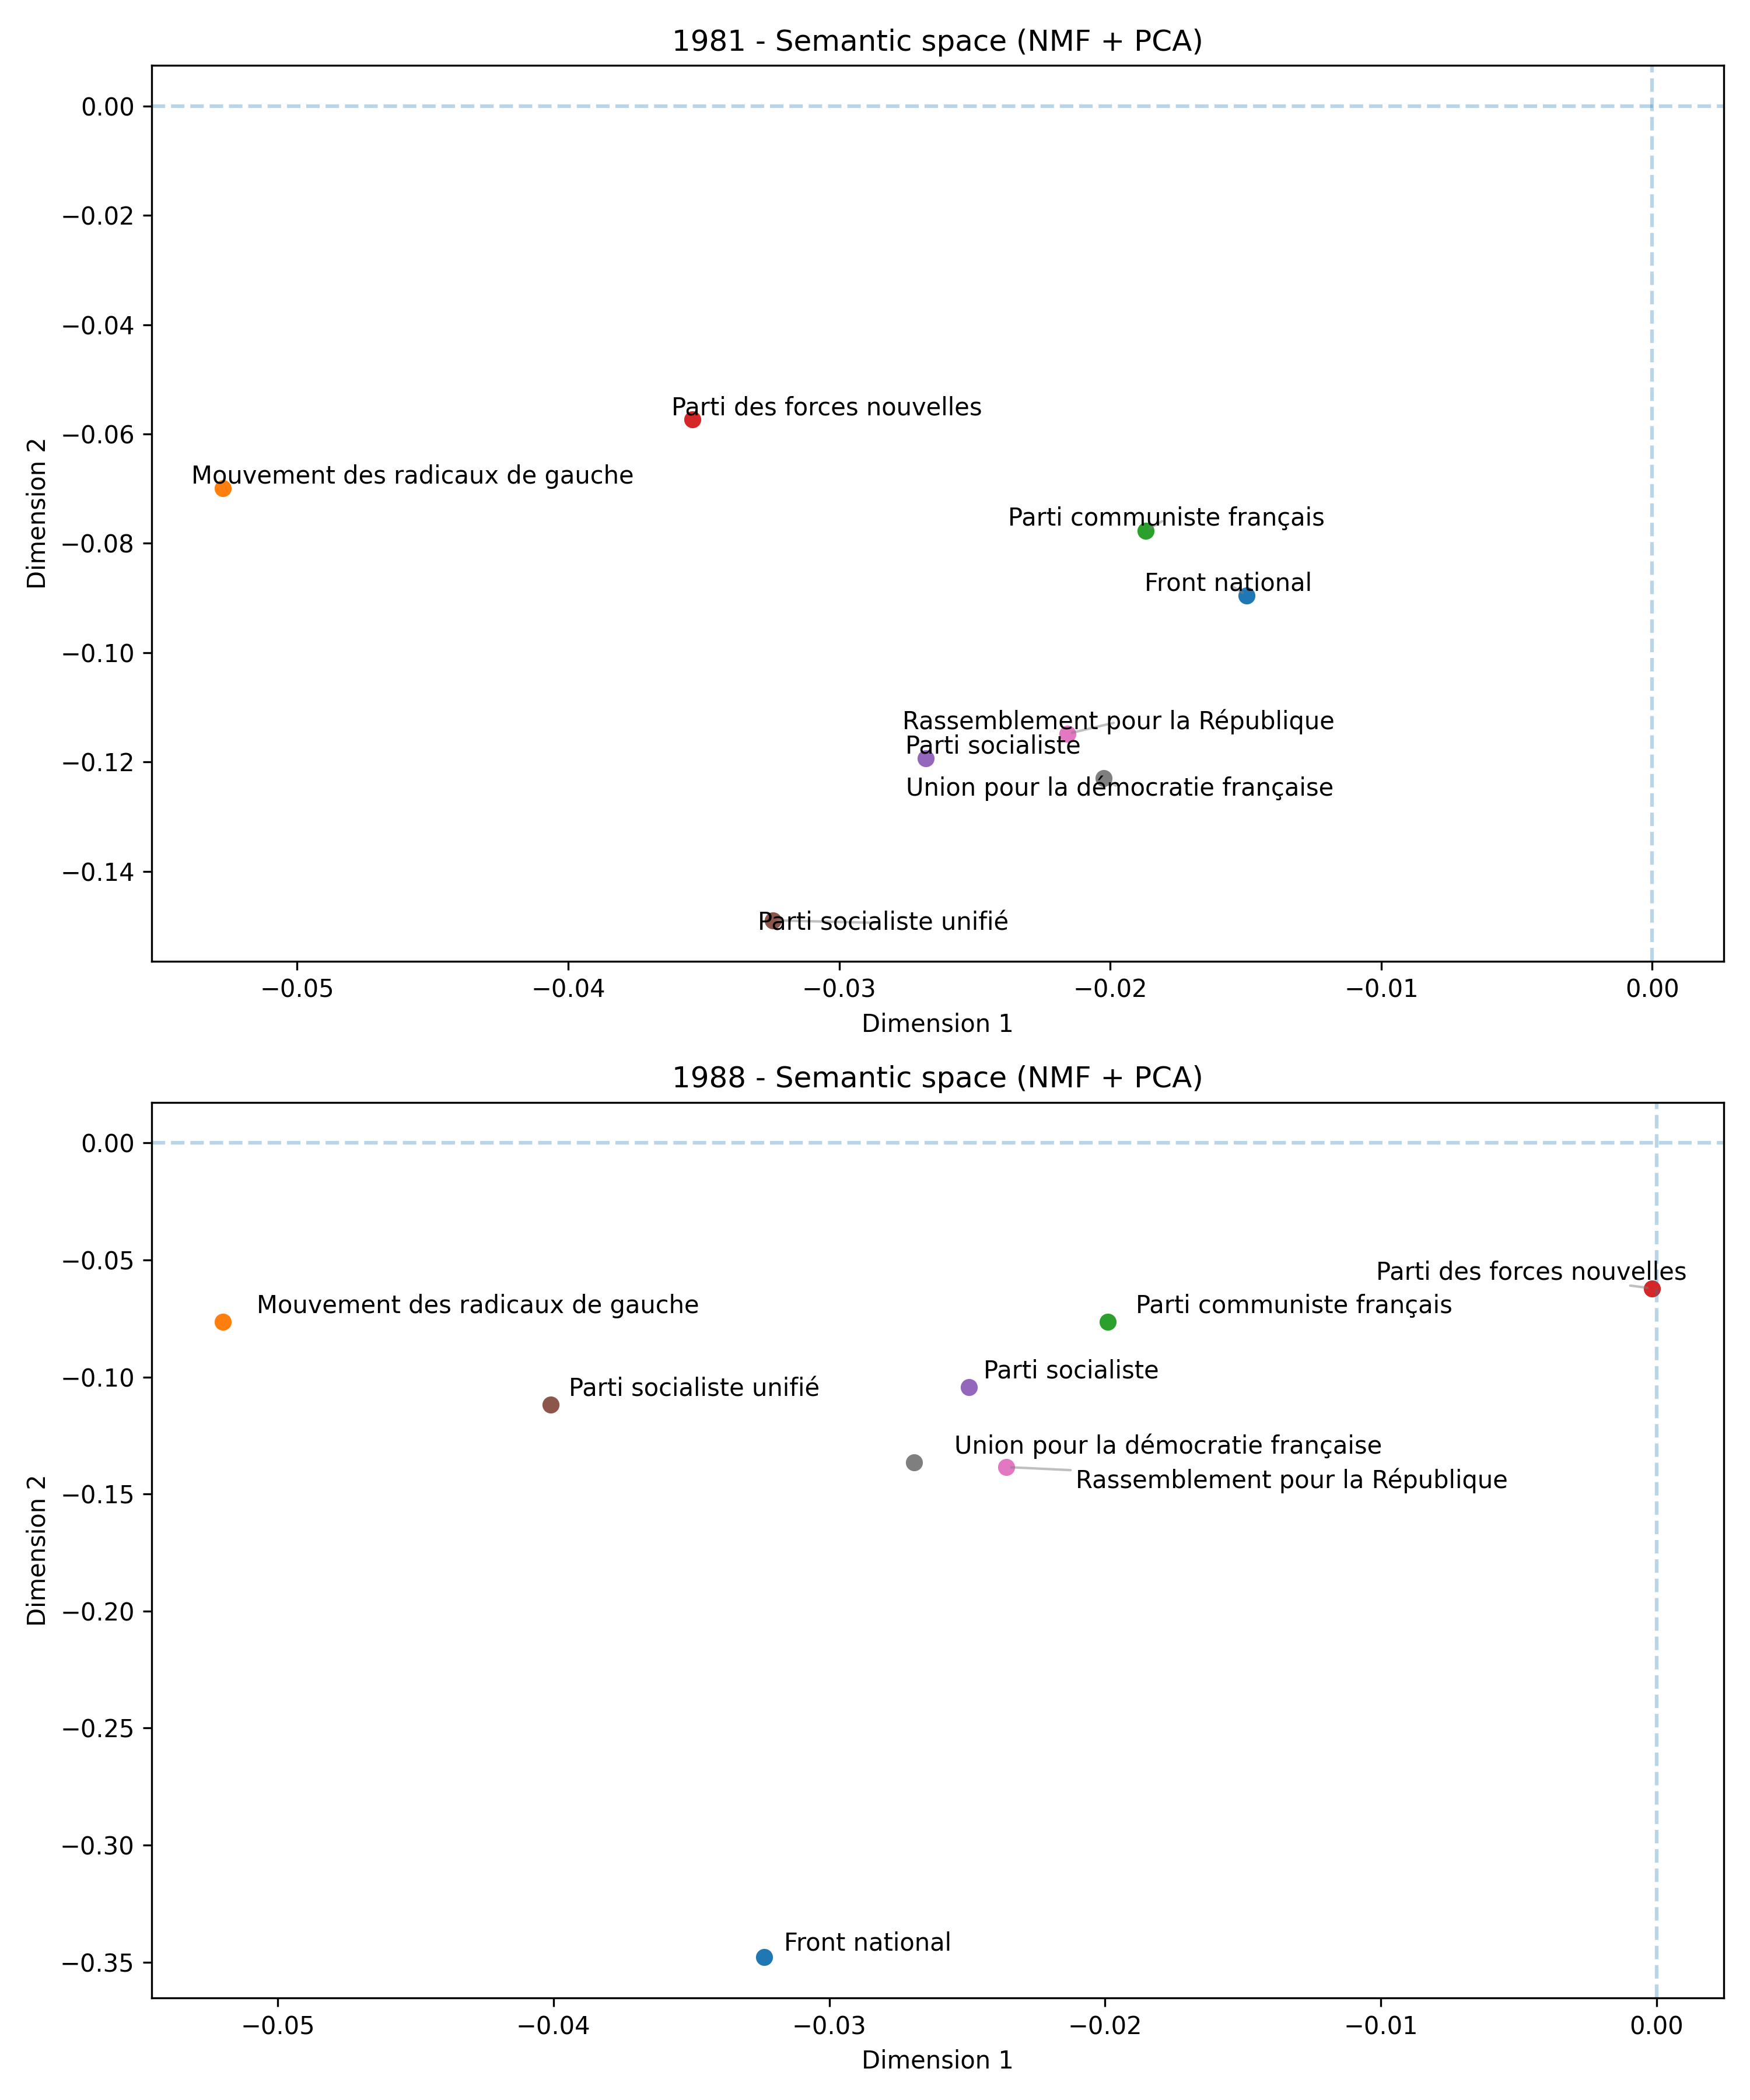
\includegraphics[width=0.8\linewidth]{nmf_pca.png}
    \caption{Projection of political parties in the semantic space (1981 and 1988)}
    \label{fig:parties}
\end{figure}

The PCA space can be interpreted as follows: \textbf{Dimension 1} opposes \textit{ideological radicalism} (e.g., autogestion, working-class left) to \textit{institutional/managerial themes} (e.g., economy, presidential majority), while \textbf{Dimension 2} captures a cleavage between \textit{left-wing ideological themes} and \textit{right-wing, national, and electoral mobilization}. Together, these axes structure the space along ideology and degree of radicalism.

Party projections (Figure~\ref{fig:parties}) exclude Lutte ouvrière and the Ligue communiste révolutionnaire (extreme positions) to focus on major parties, including the Front National.

In 1981, the space is largely bipolar: left-wing parties (PS, PCF, PSU) cluster together, while right-wing parties (RPR, UDF) form a distinct group. The Front National remains close to the traditional right. By 1988, the structure changes markedly. The Front National shifts strongly along Dimension 2, forming a distinct extreme-right pole centered on nationalism and electoral mobilization. The Socialist Party moves toward a more central, governing-oriented position, while the Communist Party remains more ideological but becomes relatively isolated. In contrast, RPR and UDF display limited movement, indicating stable positioning. Overall, the period reveals a structural transformation: from a primarily left--right opposition in 1981 to a more differentiated space in 1988, marked by the emergence of an extreme-right pole and increased fragmentation of the left.

\section{Conclusion}
Our results reveal a strong structural regularity in political communication in 1981 and 1988: despite ideological differences, party discourse is highly standardized and largely anchored in national-level political dynamics, particularly presidential elections. This suggests that legislative campaigns function less as arenas for programmatic differentiation than as extensions of presidential competition.

The analysis of the semantic space between both elections highlights important structural changes. While the 1981 political space is organized around a relatively clear bipolar left–right structure, by 1988 it becomes more fragmented. A distinct extreme-right pole emerges, driven by the Front National, which becomes increasingly isolated through a strong specialization in nationalist and identity-based themes. At the same time, the Socialist Party moves toward a more central, governing-oriented position, while the Communist Party becomes more marginal within the left-wing bloc. Right-wing parties (RPR, UDF) remain comparatively stable across the period, reflecting continuity in institutional and managerial discourse. A second key finding concerns the asymmetry between major and minor parties. While mainstream parties (PS, RPR, UDF) exhibit relatively stable and convergent thematic structures, smaller parties such as the Communist Party and the Front National display more reactive and relational discourses, systematically positioning themselves in response to dominant political actors. This highlights a form of discursive dependency, where peripheral actors structure their narratives around the main agenda.

The comparison between models highlights the importance of aligning modeling choices with textual characteristics. While BERTopic offers advantages for short and highly contextualized texts, it appears less well suited to structured and repetitive documents such as electoral manifestos. In contrast, NMF proves particularly effective in capturing temporal shifts and relative topic salience.
\newpage

\appendix

\section{Appendix: Search grid and hyperparameters}

\subsection{BERTopic} \label{app:grid_bert}

\begin{table}[htbp]
\centering
\begin{tabular}{ccccccccc}
\toprule
$n\_comp$ & $n\_neigh$ & $min\_clust$ & $min\_dist$ & $coh$ & $div$ & $score$ & $n\_topics$ & $topic0$ \\
\midrule
4 & 19 & 15 & 0.3 & 0.43 & 0.87 & 0.37 & 6 & 4716 \\
4 & 19 & 16 & 0.3 & 0.43 & 0.87 & 0.37 & 6 & 4716 \\
4 & 19 & 18 & 0.3 & 0.43 & 0.87 & 0.37 & 6 & 4716 \\
\textbf{4} & \textbf{19} & \textbf{19} & \textbf{0.3} & \textbf{0.43} & \textbf{0.87} & \textbf{0.37} & \textbf{6} & \textbf{4716} \\
2 & 19 & 15 & 0.3 & 0.43 & 0.87 & 0.37 & 6 & 4715 \\
2 & 19 & 16 & 0.3 & 0.43 & 0.87 & 0.37 & 6 & 4715 \\
4 & 19 & 17 & 0.3 & 0.43 & 0.87 & 0.37 & 6 & 4716 \\
2 & 19 & 17 & 0.3 & 0.43 & 0.85 & 0.36 & 6 & 4714 \\
2 & 19 & 18 & 0.3 & 0.43 & 0.85 & 0.36 & 6 & 4714 \\
2 & 19 & 19 & 0.3 & 0.43 & 0.85 & 0.36 & 6 & 4714 \\
3 & 18 & 14 & 0.3 & 0.44 & 0.77 & 0.34 & 7 & 4696 \\
4 & 13 & 17 & 0.5 & 0.43 & 0.77 & 0.33 & 7 & 4709 \\
4 & 13 & 19 & 0.5 & 0.43 & 0.77 & 0.33 & 7 & 4709 \\
4 & 13 & 18 & 0.5 & 0.43 & 0.77 & 0.33 & 7 & 4709 \\
2 & 18 & 17 & 0.1 & 0.47 & 0.71 & 0.33 & 9 & 4448 \\
2 & 18 & 18 & 0.1 & 0.47 & 0.71 & 0.33 & 9 & 4448 \\
\bottomrule
\end{tabular}
\caption{BERTopic grid search}
\label{tab:bertopic_grid}
\end{table}

\subsection{NMF and LDA} \label{app:grid_nmf}

\begin{table}[htbp]
\centering
\small
\begin{minipage}{0.42\textwidth}
\begin{tabular}{rrrrr}
\hline
$n\_topics$ & ngram\_range & coherence & diversity & score \\
\hline
15 & (1, 2) & 0.5787 & 0.8800 & 0.5092 \\
16 & (1, 2) & 0.5829 & 0.8688 & 0.5064 \\
17 & (1, 2) & 0.5906 & 0.8471 & 0.5003 \\
18 & (1, 2) & 0.5810 & 0.8556 & 0.4971 \\
\textbf{14} & \textbf{(1, 2)} & \textbf{0.5566} & \textbf{0.8786} & \textbf{0.4890} \\
19 & (1, 2) & 0.5738 & 0.8474 & 0.4862 \\
13 & (1, 2) & 0.5601 & 0.8615 & 0.4826 \\
12 & (1, 2) & 0.5501 & 0.8750 & 0.4813 \\
11 & (1, 2) & 0.5309 & 0.8636 & 0.4585 \\
10 & (1, 2) & 0.5191 & 0.8700 & 0.4516 \\
9  & (1, 2) & 0.5058 & 0.8667 & 0.4384 \\
8  & (1, 2) & 0.4995 & 0.8750 & 0.4371 \\
8  & (1, 1) & 0.4834 & 0.9000 & 0.4351 \\
13 & (1, 1) & 0.5102 & 0.8462 & 0.4317 \\
19 & (1, 1) & 0.5212 & 0.8263 & 0.4307 \\
9  & (1, 1) & 0.4838 & 0.8889 & 0.4301 \\
14 & (1, 1) & 0.5132 & 0.8357 & 0.4289 \\
15 & (1, 1) & 0.5139 & 0.8133 & 0.4180 \\
17 & (1, 1) & 0.5133 & 0.8118 & 0.4167 \\
12 & (1, 1) & 0.5017 & 0.8250 & 0.4139 \\
18 & (1, 1) & 0.5047 & 0.8167 & 0.4122 \\
16 & (1, 1) & 0.5112 & 0.8063 & 0.4121 \\
11 & (1, 1) & 0.4968 & 0.8182 & 0.4065 \\
10 & (1, 1) & 0.4864 & 0.8300 & 0.4037 \\
\hline
\end{tabular}
\caption{NMF grid search}
\label{tab:nmf_grid}
\end{minipage}
\hfill 
\begin{minipage}{0.42\textwidth}
\begin{tabular}{rrrrr}
\hline
$n\_topics$ & ngram\_range & coherence & diversity & score \\
\hline
18 & (1, 2) & 0.4980 & 0.7333 & 0.3652 \\
\textbf{13} & \textbf{(1, 2)} & \textbf{0.5116} & \textbf{0.7077} & \textbf{0.3620} \\
8  & (1, 2) & 0.4623 & 0.7750 & 0.3583 \\
9  & (1, 1) & 0.4783 & 0.7444 & 0.3561 \\
14 & (1, 1) & 0.4728 & 0.7286 & 0.3444 \\
10 & (1, 2) & 0.5126 & 0.6700 & 0.3434 \\
11 & (1, 1) & 0.4652 & 0.7364 & 0.3426 \\
9  & (1, 2) & 0.4971 & 0.6889 & 0.3425 \\
10 & (1, 1) & 0.4627 & 0.7300 & 0.3378 \\
11 & (1, 2) & 0.4875 & 0.6909 & 0.3368 \\
15 & (1, 2) & 0.4743 & 0.7067 & 0.3351 \\
19 & (1, 2) & 0.4610 & 0.7211 & 0.3324 \\
16 & (1, 1) & 0.4387 & 0.7563 & 0.3318 \\
17 & (1, 2) & 0.4757 & 0.6824 & 0.3246 \\
14 & (1, 2) & 0.4767 & 0.6714 & 0.3200 \\
15 & (1, 1) & 0.4740 & 0.6733 & 0.3192 \\
17 & (1, 1) & 0.4192 & 0.7588 & 0.3181 \\
18 & (1, 1) & 0.4334 & 0.7333 & 0.3178 \\
16 & (1, 2) & 0.4748 & 0.6688 & 0.3176 \\
13 & (1, 1) & 0.4690 & 0.6769 & 0.3175 \\
8  & (1, 1) & 0.4453 & 0.7125 & 0.3173 \\
19 & (1, 1) & 0.4592 & 0.6789 & 0.3118 \\
12 & (1, 2) & 0.4431 & 0.7000 & 0.3102 \\
12 & (1, 1) & 0.4471 & 0.6833 & 0.3055 \\
\hline
\end{tabular}
\caption{LDA grid search.}
\label{tab:lda_grid}
\end{minipage}
\end{table}

\newpage
\bibliographystyle{plainnat}
\newpage
\bibliography{references}


\end{document}